% This version of CVPR template is provided by Ming-Ming Cheng.
% Please leave an issue if you found a bug:
% https://github.com/MCG-NKU/CVPR_Template.

% \documentclass[review]{cvpr}
\documentclass[final]{cvpr}

\usepackage{times}
\usepackage{epsfig}
\usepackage{graphicx}
\usepackage{amsmath}
\usepackage{amssymb}

% Include other packages here, before hyperref.

% If you comment hyperref and then uncomment it, you should delete
% egpaper.aux before re-running latex.  (Or just hit 'q' on the first latex
% run, let it finish, and you should be clear).
\usepackage[pagebackref=true,breaklinks=true,colorlinks,bookmarks=false]{hyperref}


\def\cvprPaperID{****} % *** Enter the CVPR Paper ID here
\def\confYear{CVPR 2021}
% \setcounter{page}{4321} % For final version only


\begin{document}

%%%%%%%%% TITLE
\title{Learning Transformer}

\author{Zichen Tian\\
Nanyang Technological University\\
Singapore\\
{\tt\small ztian002@e.ntu.edu.sg}
}

\maketitle


%%%%%%%%% ABSTRACT
\begin{abstract}
This is a LEARNING MANUSCRIPT for me. Good to have its hyper reference function.
\end{abstract}

%%%%%%%%% BODY TEXT
\section{Background Theories}

\subsection{Self-Learning }

To distinguish between the supervised learning, self-supervised learning and unsupervised learning, check paper~\cite{liu2020self}.

Self-learning can learn the inner relationship among different components of input data. As a result, given an input that misses part of it, the self-learning can infer or complete the missing parts from the given part. For example, given the sentence "I like \underline{\hspace{0.2in}} apples.", a well-trained self-training model would complete as "I like \textit{eating} apples." because the eating are usually related with other words of the sentence, from the past learning experience.

The self-supervised learning has two features:
\begin{enumerate}
    \item Given unlabeled data, the model can generate "labels" from data itself by some data augmentation operations, e.g. rotation, crop, patching.
    \item Infer the missing information from the incomplete input.
\end{enumerate}

Self-supervised learning usually be divided into two branches~\cite{li2021multi}: 1) Generative 2) Contrastive. Generative method is trained on a pretext task (generative task) which generates pseudo label from un-annotated data. For example, in~\cite{gidaris2018unsupervised} rotates the image and predict the angle in the pretext task. By solving this pretext task, the model would learn some meaningful representations of the underlying data. These representation information would further be leveraged in another tasks. Contrastive 

\begin{figure}[ht]
\begin{center}
\fbox{
   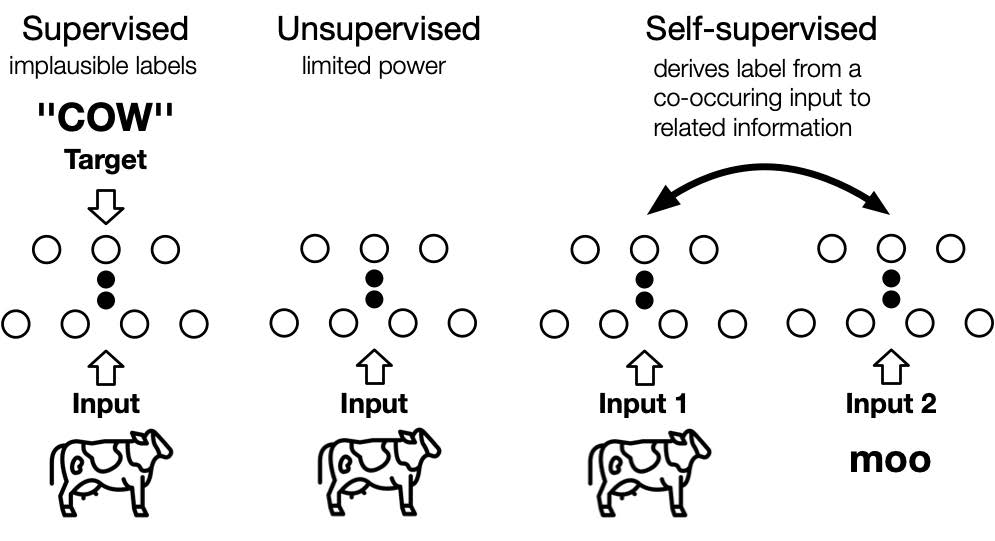
\includegraphics[width=0.9\linewidth]{images/self-supervise-compare.jpg}
   }
\end{center}
   \caption{Illustration of three types~\cite{liu2020self}. The Self-supervised learning always has the cow image and moo voice appearing altogether, which is called multi-modality.
   }
\label{fig:sscompare}
\end{figure}

Self-learning sometimes be treated as a branch of un-supervised learning~\cite{liu2020self}. But the two are different from the objective. The unsupervised learning is to do clustering, while the self-supervised learning is to dig out the relations among data and recover the missing data.

{\small
\bibliographystyle{ieee_fullname}
\bibliography{ref}
}

\end{document}
